
\subsection{Соединения с кратными связями элемент - элемент, особенности их химических свойств, структуры, электронного строения.}

Начнем рассмотрение соединений с кратной связью элемент-элемент с примера тетрахлорэтилена (молекула плоская) (рис. 1). Он образуется из двух молекул $ССl_2$ (рис.2), дихлоркарбена, которое
является производным очень высокореакционноспособных соединений - карбенов. Дихлоркарбен $CCl_2$ существует только в синглетном состоянии. Заметим, что важен трихлорэтилен - его
используют в химчистке как сухое очищающее средство, оно дешевле и лучше очищает (рис. 3).\\

Теперь посмотрим, как устроен $SnCl_2$ в газовой фазе и кристалле. Оказывается, что он не образует соединений с кратной связью, подобно дихлоркарбену, но молекулы ассоциированы донорноакцепторными связями (рис. 4).

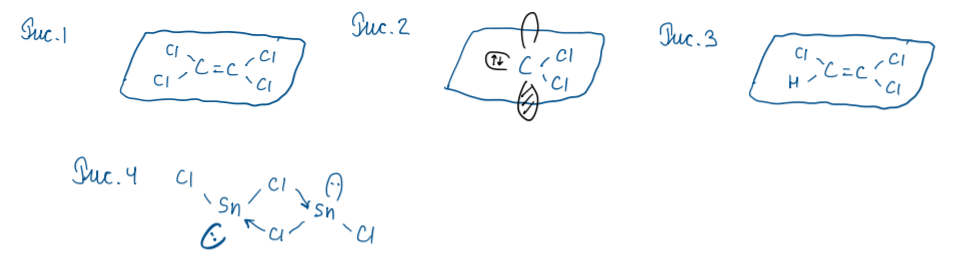
\includegraphics{images/14v1.png}

Чтобы синтезировать молекулы с кратными связями, были предложено использовать заместители: водород (ничего не получилось, быстро отказались) и такие крупные органические лиганды,
которые не способны выступить в качестве мостиковых групп.

R2Э=ЭR2
Использование органических заместителей исключает образование донорно-акцепторных связей, что характерно для соединений с мостиковыми лигандами, где нет кратных связей. В случае
использование органических заместителей возможны два варианта: либо молекула димеризуется с кратной связью, либо образует полимер с одинарными связями. То есть, в димере есть и сигма-,
и пи-связи, а в полимере лишь сигма.

Эксперименты показали, что если использовать такой маленький заместитель, как СН3, то происходит образование полимерных структур. Поэтому берут очень большие заместители. В таком
случае молекула будет существовать либо как R2Э (радикал), либо как димер, но никак не полимер из-за нарастания стерического напряжения. Такой подход к синтезу соединений называют
кинетической стабилизацией. В настоящее время известно около 30 таких подходящих заместителей. Примеры на рис. 5. Одна из схем синтеза представлена на рис. 6. 

Если посмотреть на данные по энергиям и длинам двойных связей для элементов четвертой группы, то выяснится, что выигрыш в энергии за счет образования двойной связи падает вниз по
группе, причем выигрыш у углерода сильно больше, чем у остальных элементов, и это несмотря на то, что углерод - самый маленький и, казалось бы, должны возникать стерические затруднения.
У свинца выигрыша за счет образования двойной связи вообще нет. Естественно, что длины двойных связей короче, чем длины одинарных связей, так как они прочнее (но у свинца двойная связь
длиннее).

Важно понимать, что если мы вычтем энергию одинарной связи Э-Э из энергии кратной связи Э=Э, то мы не получим энергию той «второй палочки». Это так, потому что длины двойной и
одинарной связи не равны. Чтобы отдельно вычислить энергию второй связи, надо прибегнуть к вычислительным методам квантовой химии. В таблицах, энергия связи Э=Э - это энергия, которая
отвечает тому, чтобы разорвать и первую, и вторую связь вместе, а не какую-то одну.

Получается, что соединения с кратными связями для непереходных элементов нехарактерны, исключение составляют соединения элементов второго периода. 

Если посмотреть на электронную структуру карбеноподобных частиц (рис. 7), то видно, что между элементами образуются две связи. Однако это не сигма- и пи-связь, а это две донорноакцепторные связи. Такие соединения не являются плоскими: пара заместителей одного элемента лежит выше плоскости Э=Э, а пара другого - ниже (рис. 8).

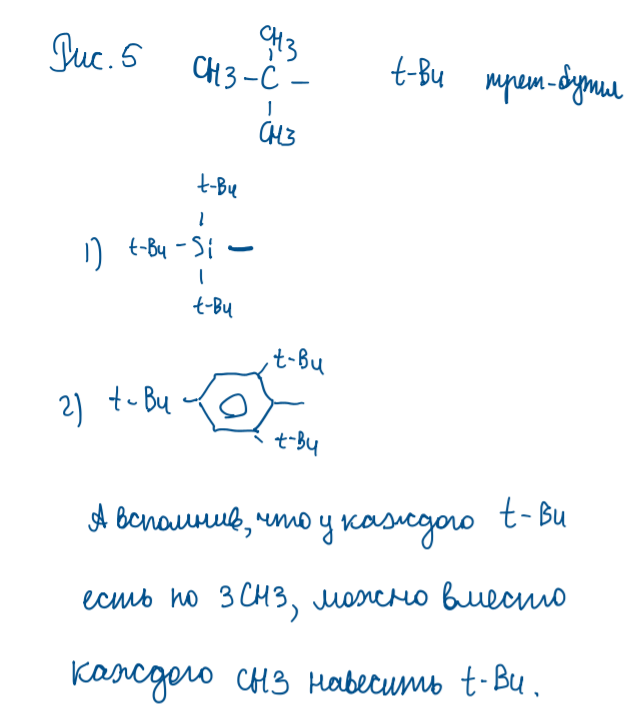
\includegraphics{images/14v2.png}

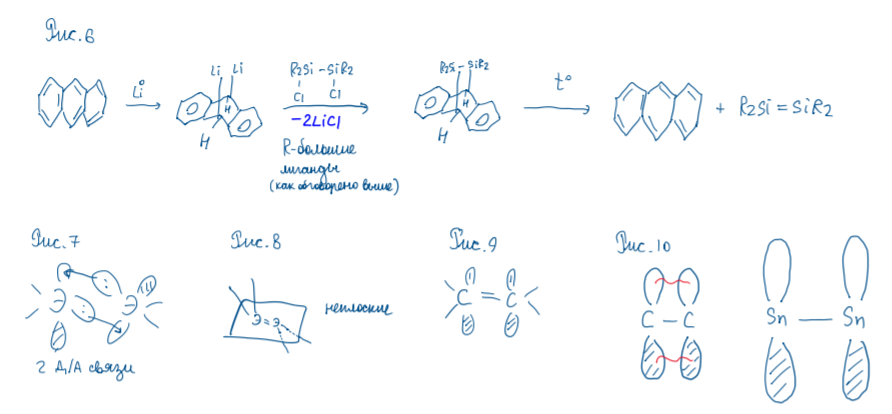
\includegraphics{images/14v3.png}

Что касается аналогичных рядов для элементов 5, 6, 7 групп, то закономерности там схожи, но это изучено гораздо меньше, потому что проще рассматривать образование кратных связей на
примере 4 группы (тут по школьной, короткопериодной таблице Менделеева)

Что касается тройных связей, то, оказывается, они известны только у углерода - это ацетилен и его производные, они линейные. Если даже пытаться оставить один заместитель у других
элементов, то там просто сохранится валентность = 2.

Дадим объяснение харатерности для углерода кратных связей. У элементов второго периода р-орбитали, направленные перпендикулярно линии связи Э-Э, достаточно толстые при короткой длине
связи. Поэтому их перекрывание хорошее. Тем не менее, для более электроотрицательных элементов (азот и кислород) их электронные пары начинают сильнее отталкиваться, что
дестабилизирует связь, делает ее энергию меньше (по модулю), несмотря на более короткие связи. Рассматривая соединения углерода, заметим, что если на р-орбиталях углерода будет по одному
электрону (рис. 9), то, за счет хорошего перекрывания, произойдет образование пи-связи. Если будет по два электрона, то они будут сильно отталкиваться, что дестабилизирует двойную связь.

Вниз по группе, важно, что р-орбитали растут в основном в длину, а в ширину почти не растут (рис. 10). Поэтому образование пи-связи не происходит, даже если электронов мало, а также тогда,
когда их много - на самом деле, эти орбитали меньше чувствуют друг друга. Так, к примеру, в молекуле S8 нет двойных связей, хотя у каждой серы есть по две НЭП. НЭП разных атомов просто
друг другу не мешают. Поскольку перекрывание там не очень хорошее, то система останавливается на образовании только сигма-связей.

Что касается химических свойств, то для соединений с кратной связью характерны реакции присоединения по двойной связи с ее разрушением; повышенной электронной плотностью двойной
связи такие соединения могут садиться на какие-нибудь акцепторные центры (рис. 11).

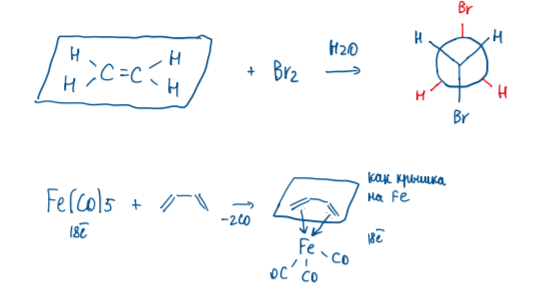
\includegraphics{images/14v4.png}
